\chapter{Application of load balancing strategies to the HP Smart Array 642}
\label{chap4:title}
\nomenclature{HP}{Hewlett Packard}
\nomenclature{VHDCI}{Very-High-Density Cable Interconnect}

This part of the thesis shows how is it possible to apply load balancing during communication between SCSI controller and disks. We discuss several strategies of sending the commands and try to estimate which one is better. Moreover, we suggest to apply a dynamic load balancing system for finding the optimal values for the erasure. That system solves our optimization Problem \ref{opt_problem}, which is the main task in this research.

\section{HP Smart Array 642}
HP Smart Array 642 is a SCSI RAID controller, which supports protocol Ultra-320 SCSI \cite{hp_642_desc}. This device has one internal and one external VHDCI (Very-High-Density Cable Interconnect) SCSI ports. The internal port gives the possibility to connect up to 6 internal disks and the external one up to 14 disks. That means that HP Smart Array 642 controller supports 20 disks. Maximum capacity for all disks in total is 6 TB. Controller has PCI-X bus, which has a 133-MHz frequency. That means that the maximum bandwidth of the bus is 1 GB/s. Moreover, the architecture is 64-bit.

The Figure \ref{fig:HP_Smart_Array_642} presents the described controller.
\begin{figure}[h]
\begin{center}
  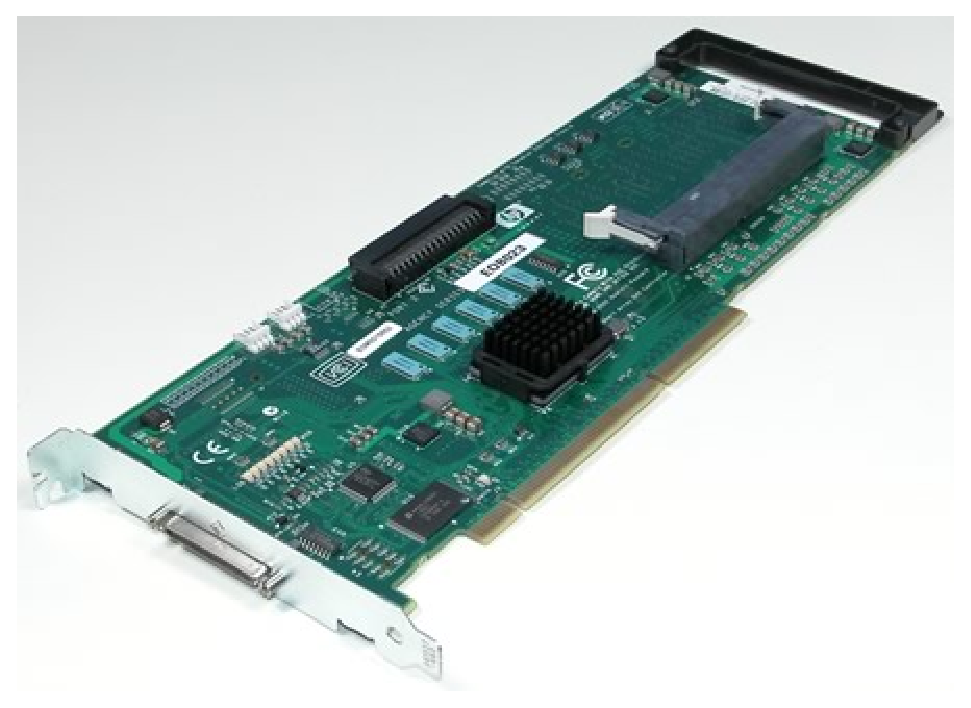
\includegraphics[width=0.65\textwidth]{HP_Smart_Array_642}
\end{center}
  \caption{HP Smart Array 642 controller}
  \label{fig:HP_Smart_Array_642}
\end{figure}


\section{Load balancing strategies}
\label{subsec:lb_strategies}

This section presents a description of the methods for solving the problem presented above in the Chapter \ref{chap3:title}. The solutions that we offer are simple, but effectively show the results in practice. We applied them for testing the erasure of several disks and find out which one is optimal. The main problem of the research is to minimize the functional of time $T$ or prove that it is not possible because of some limiting factor. That means that we try to find the fastest way of sending the write commands to the disks through the controller.

We applied three load balancing strategies during testing the erasure of the disks behind HP Smart Array 642 controller. In several papers \cite{load_bal_policy}, \cite{diff_policies} there were some discussions about strategies. Because of the specificity of the problem it was difficult to apply them in our case, but it gave an idea how it should work. First two strategies, which we applied, are sequential and the third one is parallel, which works more effectively than others. Because first two strategies are much slower than the third one, we tested them with 5 disks connected with the backplane to the internal port of the controller. The third strategy was tested with the enclosure of 14 disks connected to the external port of the controller. In both cases we chose 18.2 GB disks from Compaq. The Section \ref{sec:theory_est} discusses the theoretical expectations about these disks.

Lets consider the strategies in more detail. The first strategy performs the complete erasure disk by disk. That means that until we do not erase the current disk the program does not start the erasure of the next disk. From the Section \ref{sec:theory_est} we know that for the erasure one 18.2 GB disk we need to send 582 WRITE SAME 10 commands. According to the point that for testing first strategy we took 5 disks we get the following matrix $H_{s1}$ from the Model \ref{eq:load_balancing_matrix} for complete erasure:
\begin{equation}
	H_{s1} =
	\begin{pmatrix}
		582 & 0 & 0 & 0 & 0\\
		0 & 582 & 0 & 0 & 0\\
		0 & 0 & 582 & 0 & 0\\
		0 & 0 & 0 & 582 & 0 \\
		0 & 0 & 0 & 0 & 582 \\
	\end{pmatrix}
\end{equation}
From the matrix $H_{s1}$ we can conclude that first strategy has only 5 steps in the algorithm.


Second strategy sends one command per disk and then changes the disk. That means that in this case
matrix $H$ is completely different:
\begin{equation}
\setcounter{MaxMatrixCols}{13}
	H_{s2} =
	\begin{pmatrix}
		1 & 0 & 0 & 0 & 0 &&  		1 & 0 & 0 & 0 & 0 \\
		0 & 1 & 0 & 0 & 0 &&  		0 & 1 & 0 & 0 & 0 \\
		0 & 0 & 1 & 0 & 0 &\ldots&   0 & 0 & 1 & 0 & 0 \\
		0 & 0 & 0 & 1 & 0 &&  		0 & 0 & 0 & 1 & 0 \\
		0 & 0 & 0 & 0 & 1 &&  		0 & 0 & 0 & 0 & 1 \\
	\end{pmatrix}.
\end{equation}
For the second strategy the dimension of matrix $H$ is $5\times2910$. Value $2910$ came from multiplication of number of disks and number of commands that we need to send for the erasure. From the logic of sending commands the devices should be changed quite often, which can be a disadvantage of this strategy. 


The third strategy is using parallel computing, which makes the process for complete erasure much faster. The application creates separate thread for each disk and start sending WRITE SAME commands to that disk. It is obvious that during increasing the amount of disks the value of functional of time will increase too, but slowly, because threads are working completely separately. However, important limitations are the speeds of the disks and the bus. We can see from Figure \ref{fig:conn_model} that separate buses $c$ give the possibility to send data from the controller $b$ to the disks $d$. In our situation, only one bus $c$ exists, which is connected to the enclosure containing several disks. If we write information in parallel to several disks the bus speed can be the limitation for data transfer. The maximum speed of the current bus is 320 MB/s. For the third strategy it is difficult to present matrix $H$, because we do not know in which order WRITE SAME commands come to the disks.


\section{Planning dynamic load balancing system}
\label{subsec:plan_load_bal}

During whole research we try to find the optimal parameters for sending write commands to the disks, but it seems that our conclusions about them can be wrong before some testing or special calculations. As we mentioned in the beginning of the paper, load balancing system should take care of these things. Lets discuss what kind of static and dynamic load balancing systems we could provide for our situation. There are so many parameters which depend on the speed of erasure that it is much better to use dynamic load balancing system. However, it is also possible to apply static load balancing system using some special conditions. Currently we consider the situation when we send WRITE 10 commands to several disks using the parallel strategy. We do not take in consideration WRITE SAME command, because the bottleneck is the bus in this case and we cannot influence on that.

Main condition that we should focus on is knowledge about the cache of the controller. If we know this parameter before the erasure process it is possible to calculate the optimal buffer and optimal number of disks for erasure. The problem is that getting cache from the controller is very specific task and sometimes maybe even impossible one. However, we can manually find the maximum value for the transfer buffer inside the Linux driver. In our situation for the HP Smart Array 642, which uses the driver cciss, this value is defined as $MAX\_KMALLOC\_SIZE (4096*512)$, which means that the maximum buffer can not be larger than 2 MB. We do not know exactly if it is cache, but the value looks quite similar to the cache size. If we consider this value as cache we can calculate what is the closest value for the transfer length to the optimal one using several disks:
\begin{equation}
\label{eq:optimal_length}
	\frac{MAX\_BUFFER}{SECTOR\_SIZE*MAX\_DISKS} 
\end{equation}
% = \frac{4096*512}{512*14} = 292.57.
In our case we send the buffer with the value of power of two, that is why we should find the value, which is closest from the bottom, otherwise we exceed the cache size. If we consider 14 disks, we can see that the value $4096*512/512*14=292.57$ is closest to 256. Blancco software sends the buffer exactly with the transfer length 256, but it is optimal only when the number of disks is more than 8. Lets calculate the transfer length in case that we have 8 disks: $4096*512/512*8 = 512$.
%\begin{equation}
%	\frac{4096*512}{512*8} = 512.
%\end{equation}
This fact explains that we should use another transfer length to get an optimal way of sending commands. Moreover, we understand that for 4 disks we need 1024 and for 2 disks - 2048. We proved this theory by making several tests. The Figure \ref{fig:comp_256_best_length} shows that if we base on our theory Blancco software sends the optimal buffer only for disks 9-14. If we have less than 9 disks in the enclosure, we can erase them faster using another transfer length.

Based on our theory if we have 9 disks and transfer length is 512, the buffer will exceed the limit of 2 MB and the erasure process should go slower than with transfer length 256. However, in practise, the results of testing show that even for disks 9-14 the buffer with transfer length 512 allows to erase the devices faster than with transfer length 256. The Figure \ref{fig:comp_256_best2_length} explains it more clear. From these results we could make a conclusion that some other parameters, that we did not include, influence on the speed. Anyway, suggested static load balancing system helps to improve the erasure, which gives a possibility to do it faster than Blancco software currently does. Moreover, if we base on the testing results, we could provide even faster load balancing system.

In some versions of Blancco software it is possible to add disks during the erasure process. In this case our static load balancing system should recalculate the optimal transfer length and set it correctly to the commands during the erasure process. From the programming point of view it could be difficult to access the function, which performs the erasure, but not impossible. If we cannot influence on the transfer length of the currently working disks, it could be better to wait until the application erases them, because the bus can be already filled completely. So, if we decide to add more commands because of new disks, we could come to the situation that the commands will stay in the queue before coming to the bus. It can make the speed of the erasure much slower.

If we consider the situation that we can influence on the transfer length during the erasure process, we get that our static load balancing system transforms to the dynamic load balancing system. The purpose of this load balancing system is to calculate and set the optimal transfer length for the write command depending on the amount of disks. In the situation of ending the erasure this load balancing system can help us one more time. Of course, that if we have disks, which have the same size and rotation speed, there is no reason to make any more calculations for searching the optimal parameters after some disks are erased, because the time should be almost equal to each other. But if we have disks with the different capacities, it makes sense to set another transfer length after some disks are erased. That means that suggested dynamic load balancing system should work in three situations:
\begin{enumerate}
	\setlength{\itemsep}{-2mm}
	\item Before the erasure
	\item During the erasure, when some disks are added or stopped
	\item After some disks finish the erasure
\end{enumerate}

However, if we consider the situation that the optimal value was found and look to the Figure \ref{fig:compare_write_10_14disks} we can notice that the maximums of 2 curves belongs to different disks. It gives an idea that not only speed of the disk and buffer length influence on the erasure speed. It could be possible to find the way of sending commands, which will give the medium time of all disks, but it can be difficult because for each disk a separate thread exists. This medium time will give us a great advantage, because the time for complete erasure will decrease and it will be almost equal for all disks. Moreover, our load balancing system will not need to analyse the optimal transfer length for last disks, which do not finish the erasure yet.

One of the possible ways of trying to find the medium time is to analyse each thread. For example, we can make that each thread will return the percentage of process with some step. Using this value we can analyse which disk works faster or slower. After that the dynamic load balancing system stops the erasure process for some fast disks. Thus, we will get some free space in the bus and could increase the transfer length for the slow disk. This action could give us an advantage if the limit is not a disk speed. After the next returns from the threads if the result of the slow disk is larger than fast disks we turn on the erasure for all disks. Because user is allowed to stop or add disks this strategy can give several problems for the software developer.

